The scalability of Earth System Models (ESMs) is the leading target of the 
\href{http://www.dkrz.de/Klimaforschung/dkrz-und-klimaforschung/infraproj/scales
}{ScalES}
project, in particular with regard to future computer development. Our work  
focuses on overcoming the I/O bottleneck.  The 
\href{https://code.mpimet.mpg.de/projects/cdi}{Climate Data Interface} ({\CDI}) is a 
sophisticated data handling library of 
the Max-Planck-Institute for Meteorology with broad acceptence in the 
community. 
\begin{wrapfigure}{r}{.4\textwidth}
\vspace{-10pt}
\centering
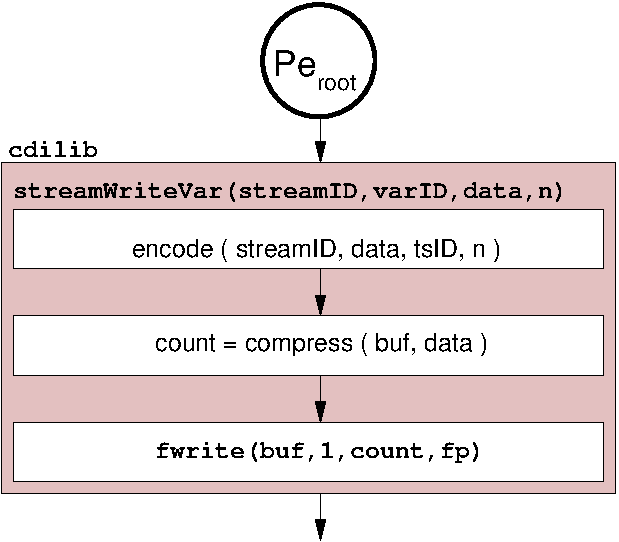
\includegraphics[scale=0.5]{../graphics/serial.pdf}
\vspace{-10pt}
\caption{{{\CDI} {\tt streamWriteVar}}}
\vspace{-10pt}
\end{wrapfigure}
Its I/O is carried out synchronously relative to the model calculation. 
We have decided to parallelize the file writing with the {\CDI}, because of the 
great benefit for many ESMs.
\smallskip 
 
We analyzed 
some HPC systems concerning the impact of their architecture, filesystem and 
MPI implementation on their I/O performance and scalability. The investigation 
delivered a large spectrum of results. As a consequence, 
we introduce different modes of low level file writing. The tasks 
of the I/O processes, which are now decoupled from the model calculation, are split.
We destinguish into collecting the data, encode, compress 
and buffer it on one side and writing the data to file on the other. The extension 
of the {\CDI} with parallel writing ({\pio}) provides five different I/O modes 
making use of this role allocation. The modulation of I/O mode, numbers and 
location of processes with the best performance on a 
special machine can be determined in test runs. 
\smallskip  

On some systems it is impossible to write from different physical nodes to one 
file. Taking the architectural structures into consideration we made a key 
pillar for the design of {\pio} from the distribution of I/O processes and files 
on physical nodes. If the I/O processes are located on different physical nodes, 
the {\tt MPI} communicator for the group of I/O processes is split and each 
subgroup gets a loadbalanced subset of the files to write. On some machines 
this approach increases the throughput remarkably.
\smallskip 

The application programming interface of the {\CDI} is kept untouched, 
we introduce only a few indispensable functions and encapsulate the other 
developments inside the library. The models have to eliminate the special 
position of the root process with respect to file writing. All model processes 
``write'' their chunk of the decomposed data and save the time former needed 
for gathering and low level writing. 